\section{Introduction}
Since Rutherford’s discovery of the nucleus in the early 19th century,\cite{noauthor_discovery_nodate} nuclear physics has been an intense area of research and has led to many discoveries from the neutron in 1932 by James Chadwick \cite{noauthor_discovery_nodate-1} and later the strong force to nuclear fission and its capabilities as a method to produce low carbon electricity.
The nucleus is composed of two fermions (proton and neutron) with similar mass and is held together by the strong nuclear force.
The letter Z is used to denote the number of protons, while the letter N is used to denote the number of neutrons in an atom. The positively charged protons determine most of the chemical properties of the atom – changing the Z number will produce a different element. Atoms with the same Z number but different N number are known as isotopes of that element.

The nuclear landscape can be characterised by \cref{fig:intronuclan}, known as the ‘Segrè Chart’ where every proton (Z) and neutron (N) combination for each discovered nuclide is represented.
There are theoretically over 7 000 isotopes predicted to exist and of which only around a half have been discovered (either in nature or in the lab) \cite{erler_limits_2012}.
The 288 stable isotopes are shown in black in what is known as the ‘valley of stability’.
Moving further from this valley by adding protons or neutrons, the unstable isotopes with a half-life shorter than the expected lifetime of the solar system are represented in the rest of the pixealated graph [7].
In light blue are shown the predicted proton (upper line) and neutron (lower line) driplines, beyond which the strong force can no longer bind more nucleons to the nucleus \cite{noauthor_amazing_nodate}.
Exploring these driplines and discovering neutron/proton rich isotopes allows the strong force to be better understood.

The binding energy is the energy required to separate the protons and neutrons.
We can determine the binding energy from its rest mass using Einstein’s famous equation $E=mc^2$.
A bounded system has a smaller mass than its separated parts.  Work is done to separate the systems; therefore, energy is put into the system.
When separated, the particles are at rest.
Consequently, if we can measure the rest mass, we would find that the rest mass has increased \cite{noauthor_binding_nodate}.
We find that the binding energy value is approximately proportional to the number of nucleons for any nucleus when looking at the binding energy.

\begin{figure}[H]
    \centering
    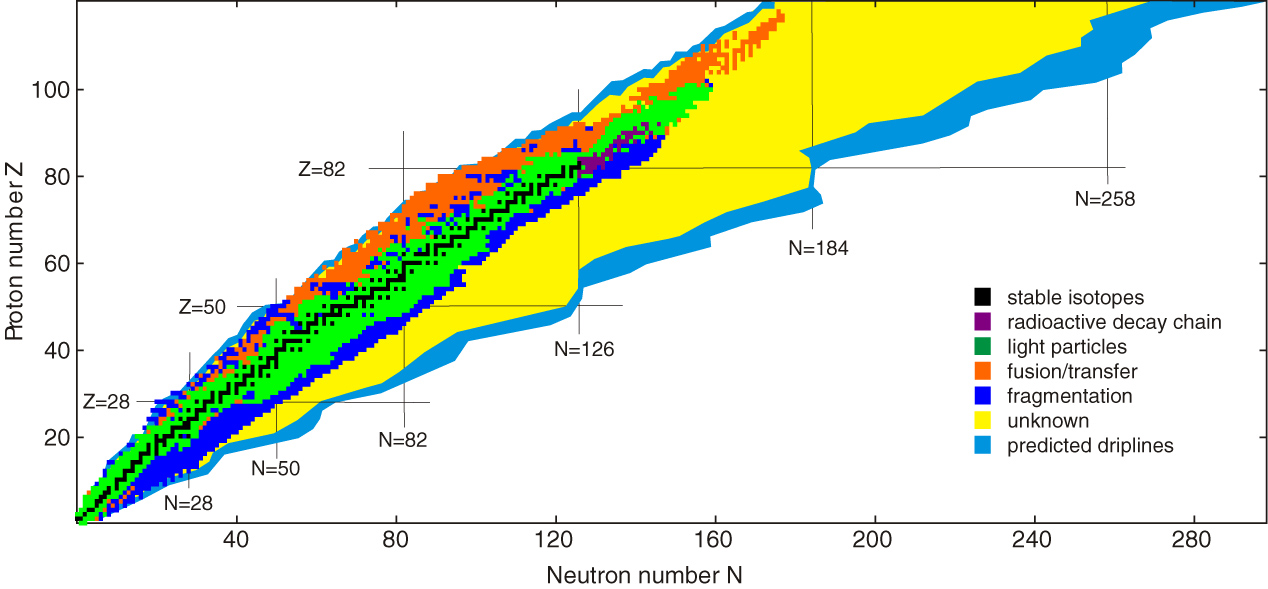
\includegraphics[width=.48\textwidth]{images/Intro_nuclearlandscape.jpg}
    \caption{The Segrè Chart visualising the nuclear landscape highlighting how the stability varies.\cite{famiano_nuclear_2019}.}\label{fig:intronuclan}
\end{figure}